%%%%%%%%%%%%%%%%%%%%%%%%%%%%%%%%%%%%%%%%%%%%%%
%                insertmeeting
% 1) Title (something creative & funny?)
% 2) Date (MM/DD/YYYY)
% 3) Location (ex. Hagerty High School)
% 4) People/Committees Present 
% 5) Picture 
% 6) Start Time & Stop Time (ex. 12:30AM to 4:30PM)
%%%%%%%%%%%%%%%%%%%%%%%%%%%%%%%%%%%%%%%%%%%%%%
\insertmeeting 
	{Illuminating Lidar} 
	{02/07/23} 
	{Hagerty High School}
	{Karissa, Laura, Tyler,  Samantha, Nathan, Robert, Jensen}
	{Images/RobotPics/robot.jpg}
	{2:30 - 4:30}
	
\hhscommittee{General}
\noindent\hfil\rule{\textwidth}{.4pt}\hfil
\subsubsection*{Goals}
\begin{itemize}
    \item Connect with a local STEM professional
    \item Update sponsor brochures and letters 
    \item review the Leagues Portfolio
    \item continue to correct errors in the notebook and add more pictures

\end{itemize} 

\noindent\hfil\rule{\textwidth}{.4pt}\hfil

\subsubsection*{Accomplishments}
Today, we met with a STEM professional named Sandro Silva, an engineer from Luminar Technologies, a company that develops vision-based lidar, mostly for self-driving cars. We talked to him about how he went about solving engineering-related problems and reaching his goals. His method of achieving goals starts with figuring out where you are, then determining where you want to be, then establishing milestones, the steps you must complete to get there. We also discussed how lidar technology works, learning that it uses laser scanning to create a highly accurate 3D map of the surroundings. The software committee showed him the OpenCV vision software that we use for our robot, which is somewhat comparable to lidar technology. Before he left, he complimented us on our commitment, effort, and hard work, telling us how impressed he was with how much time we spent on robotics. Later, the hardware committee CADed a new grip for the pole on the intake. We took a look at the newly printed battery holder in comparison to the robot and determined it would be a bit too big, so we’ll need to make it a little smaller. 

 
\begin{figure}[htp]
\centering
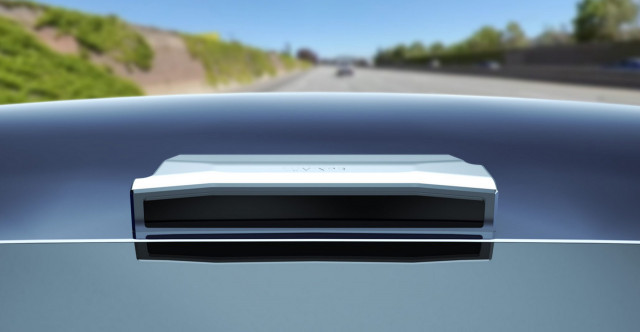
\includegraphics[width=0.95\textwidth, angle=0]{Meetings/February/02-07-23/luminar-iris-roof-mounted-lidar_100767931_m.jpg}
\caption{Luminar's lidar technology for self-driving cars}
\label{fig:pic1}
\end{figure}

\begin{figure}[htp]
\centering
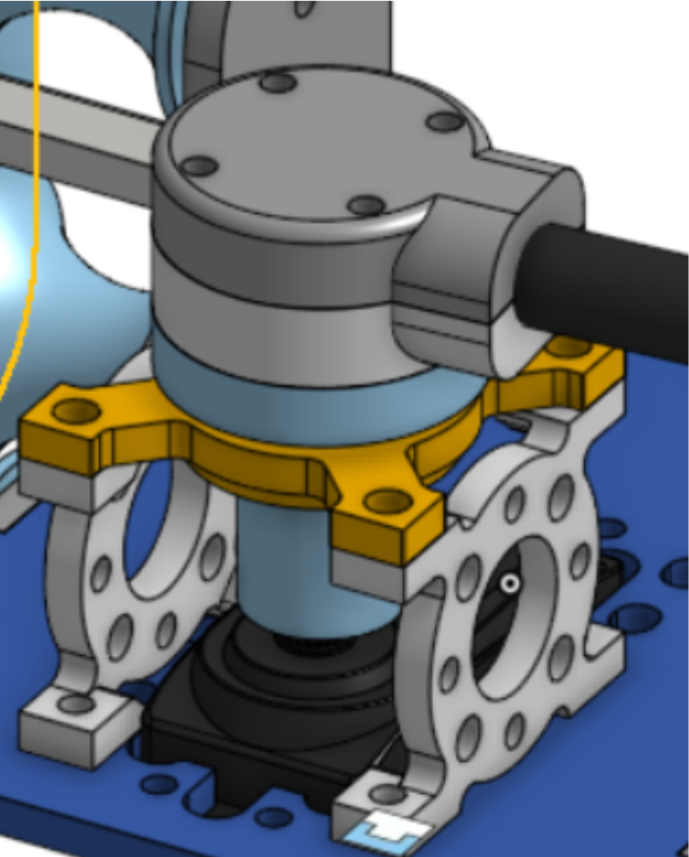
\includegraphics[width=0.95\textwidth, angle=0]{Meetings/February/02-07-23/2-7-23_CAD.PNG}
\caption{CAD for the grip intake}
\label{fig:pic2}
\end{figure}

\begin{figure}[htp]
\centering
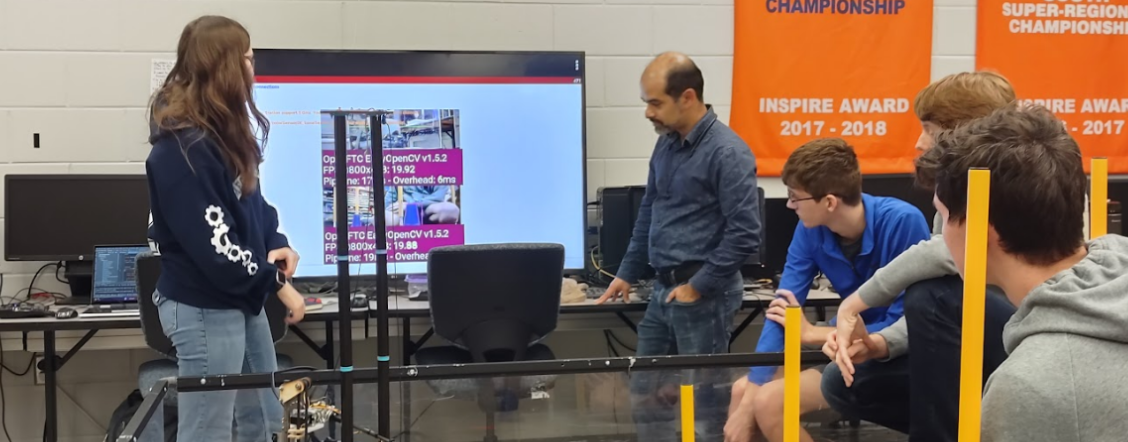
\includegraphics[width=0.95\textwidth, angle=0]{Meetings/February/02-07-23/luminar_guy.PNG}
\caption{Demonstrating our OpenCV}
\label{fig:pic3}
\end{figure}

\whatsnext{
\begin{itemize}
    \item Schedule Operation Paperback packaging
    \item Update the list of pit supplies for States
    \item Make the battery holder smaller
\end{itemize} 
}

